\section{StochEvent Class Reference}
\label{classStochEvent}\index{StochEvent@{StochEvent}}
Inheritance diagram for StochEvent::\begin{figure}[H]
\begin{center}
\leavevmode
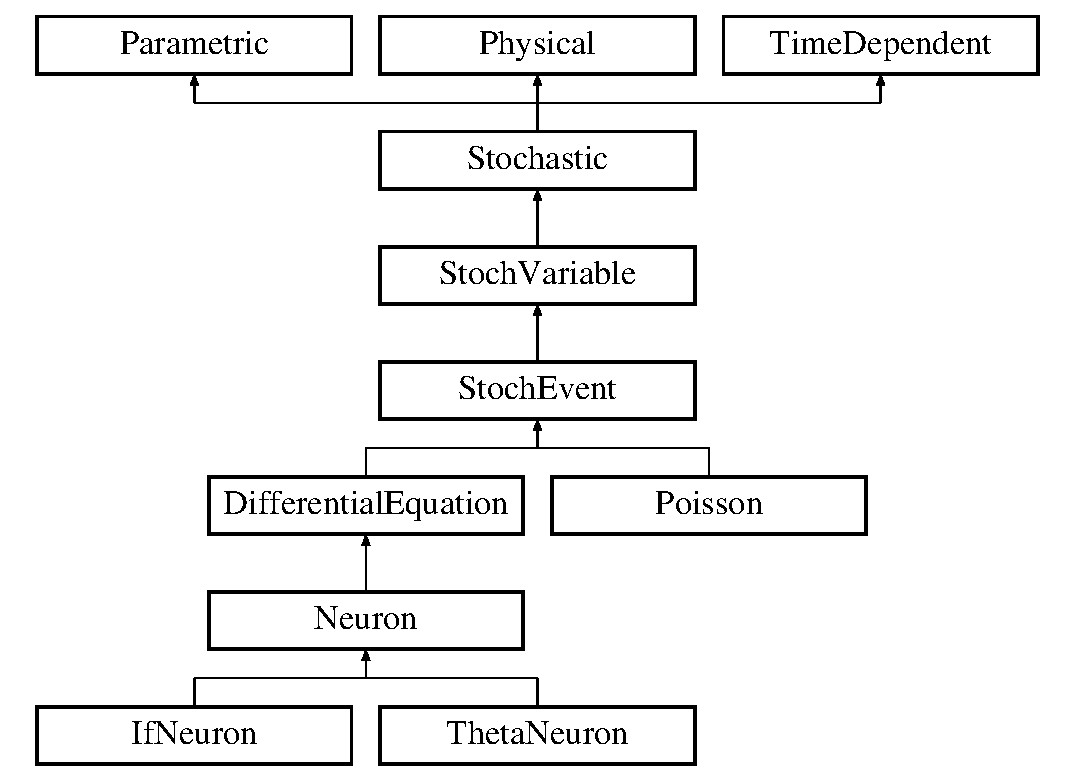
\includegraphics[height=7cm]{classStochEvent}
\end{center}
\end{figure}


\subsection{Detailed Description}
An object which generates events. 

Useful for event-triggered averages. \subsection*{Public Member Functions}
\begin{CompactItemize}
\item 
{\bf StochEvent} (class {\bf Time} $\ast$time, string name=\char`\"{}\char`\"{}, string type=\char`\"{}event\_\-generator\char`\"{})\label{classStochEvent_99d66e994628703184df39cda702f928}

\begin{CompactList}\small\item\em Create. \item\end{CompactList}\item 
virtual {\bf $\sim$StochEvent} ()\label{classStochEvent_da007eb19a6e9b5284fde1676547b191}

\begin{CompactList}\small\item\em Destroy. \item\end{CompactList}\item 
virtual bool {\bf hasEvent} ()\label{classStochEvent_d417ae021361ede47dfc6b1d65c28a75}

\begin{CompactList}\small\item\em Whether an event is present. \item\end{CompactList}\end{CompactItemize}
